\chapter{Introduction}\label{ch:introduction}
% ======================================================================================
\section{Motivation}
Fluid-structure interaction (FSI) problems play an important role in many scientific and engineering fields, such as automotive, aerospace, and biomedical industry. Despite the wide application, a comprehensive study of FSI systems still remains a challenge due to their strong nonlinearity and multi-physics nature. For most FSI problems, analytical solution of responses are not available, and physical experiments are limited in scope, expensive to conduct, and time consuming. Therefore, in order to get more insight in the physics involved in the complex interaction between fluids and solids, numerical simulations are typically used. The numerical solutions are conducted using Computational Fluid Dynamics (CFD) models for the flow field and Finite Element Analysis (FEA) for the structural response. Nevertheless, the prohibitive amount of computations has been one of the major issues in the design optimization of such coupled multidisciplinary systems. The other bottle neck is generating an appropriate computational domain that represents the fluid and solid regions with desired fidelity. The effort and time required to take a geometry from a CAD package, refining the model and generating a computational mesh is usually a large portion of the overall human time required for the simulation. This cannot be automated for complex and moving domains. Therefore, techniques that decouple the mesh topology from the shape of the solid boundary can drastically simplify the simulation of flow over complex bodies. The Immersed Boundary (IB) method addresses these challenges for complex body shapes by introducing a new approach to define the solid boundaries.

In aerospace and automotive systems, configurations are optimized for achieving maximum performance and design targets. Due to the large amount of computations involved in the FSI simulation, the gradient based methods are the best candidates for design optimization of such problems. Sensitivity analysis is the integral part of gradient based methods. Although there are analytical techniques for efficient and accurate sensitivity calculation, they have not been implemented in commercial CFD packages. Therefore, most gradient optimization techniques depend on finite difference method for sensitivity calculation when solving FSI problem. It is well known that finite difference suffers from low accuracy and high cost.

The motivation for the research proposed in this document is in two areas. First, we want to have sensitivity analysis capabilities that can treat the CFD solvers as black-box. This means that we can solve both the governing equations and the sensitivity response using the same code. Second, a robust analysis technique for the coupled FSI system based on IB method is formulated. The current approach of IB is not suited for the sensitivity analysis due to the discontinuities in its formulation. This will be explained in more detail in the following Chapters.

% ======================================================================================
\section{Literature Review}
% ---------------------------------------------------------------------------------------------
\subsection{Sensitivity Analysis}
Sensitivity analysis consists of computing the derivatives of the solution of the governing equations, i.e. the sensitivity of displacement, velocity, or pressure with respect to one of the several independent design variables, i.e. shape of boundaries or cross-sectional and size of elements. There are various applications for sensitivity information such as aircraft trajectory optimization \cite{sridhar2011aircraft}, improving the accuracy of surrogate models as in gradient enhanced Kriging \cite{han2013improving} or quantification of uncertainty \cite{pettit2004uncertainty}. However, our main motivation is the use of this information in gradient-based optimization. The calculation of gradients is often the most expensive step in the optimization cycle therefore, efficient methods for accurate calculation of sensitivities are vital to the optimization process. As shown in Figure \ref{fig:C1_sensitivityTaxonomy}, methods for sensitivity calculation can be put into three major categories: i) numerical, ii) analytical, and iii) automatic differentiation.

\begin{figure}[H]
	\centering
	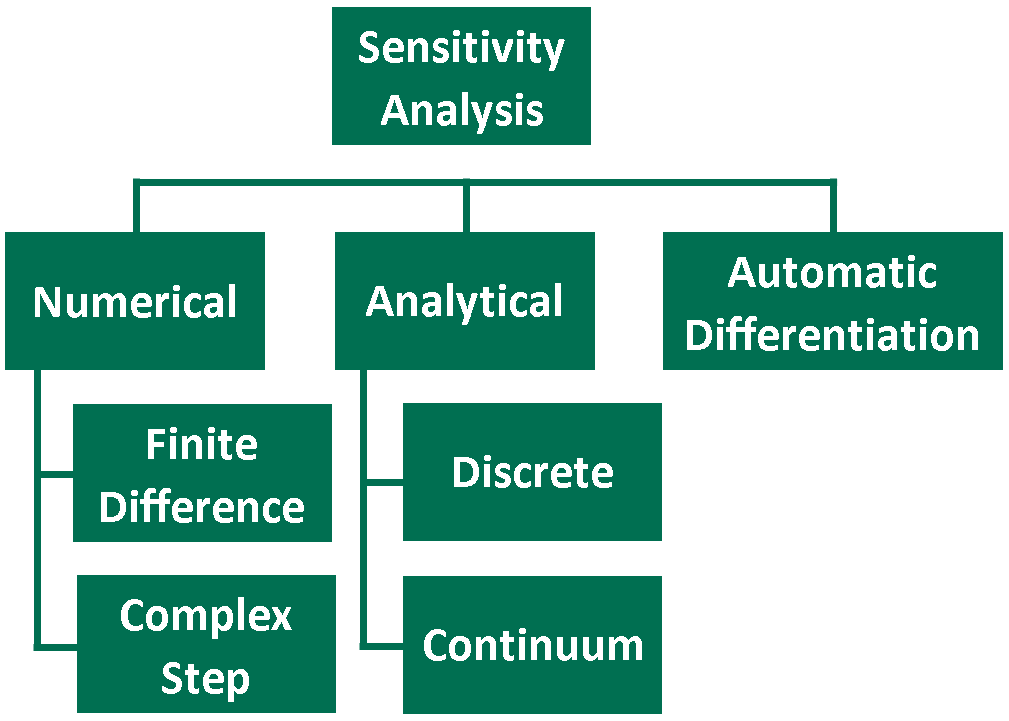
\includegraphics[height=7.00cm]{Chapter_1/figure/sensitivity_taxonomy.png}
	\caption{Sensitivity calculation techniques.}
	\label{fig:C1_sensitivityTaxonomy}
\end{figure}

The Finite Difference (FD) method is probably the easiest method to implement using a commercial software for calculating the sensitivity of a variable. The fact that they can be implemented even when a given computational model is treated as a black box makes most gradient based optimzation algorithms perform finite differences by default when the user does not provide the required gradients. However, the computational cost associated with finite difference scheme for large systems can become very high. For a system with $n$ number of design variables, the analysis has to be performed $n+1$ times to calculate the design sensitivities. Furthermore, to ensure the accuracy, convergence study needs to be done for selecting the appropriate step size for the finite difference. The inaccuracy of finite differencing could result in convergence difficulties and inaccurate optimum results \cite{sobieszczanski1997multidisciplinary}.

Complex Step (CS) method avoids the loss of precision in finite differences approximation by employing complex arithmetic \cite{martins2003complex}. The complex step derivative is defined as shown in Equation \eqref{eq:C1_compelxStepFormula}.

\begin{equation}\label{eq:C1_compelxStepFormula}
	\mathcal{F}^\prime\left(u; b\right) = \frac{\text{Im}\left[ \mathcal{F}\left(u; b + ih\right) \right]}{h}
\end{equation}

where $\mathcal{F}\left(u; b\right)$ is the function of interest such as the airfoil lift that depends of a response variable, $u$ i.e. free-stream velocity, and design variable, $b$ i.e. shape of the airfoil. Complex step approximates the sensitivities by perturbing the design variable by an imaginary value of $ih$ and then evaluating
the imaginary portion of the resulting response. Using the complex step method, we can choose a
small step size for $h$ without loosing accuracy due to no subtraction involved in CS formulation. However, many commercial packages such as ANSYS or NASTRAN cannot handle complex arithmetic which makes the implementation of complex step method infeasible. Moreover, the high cost of finite difference is still associated with the complex method as well.

Automatic differentiation (AD) is based on the systematic application of the differentiation on computer programs \cite{naumann2012art}. In the AD approach, the chain rule of differentiation is applied to every line in the program assuming that the computer program consists of a sequence of explicit functions that act successively on some variables. Therefore, by differentiating each of these functions and applying the chain rule, it is possible to calculate the sensitivities. 

There has been extensive research on utilizing AD for optimization. Bischof et al. used AD for calculating the sensitivities using a CFD solver. They used ADIFOR for differentiating the source code of their CFD code (TLNS3D) which later used for calculating the sensitivity of a transonic flow to change in the boundary conditions. Hascout et al., also used AD for a sonic boom reduction under a supersonic aircraft. In all of these works in order to implement AD, it is needed to have access to the source code and modification of the solver extensively to calculate the sensitivities. This make the use of this method for commercial codes impractical since the source code is usually not available.

The short comings of numerical and AD techniques, demands for more sophisticated methods for sensitivity calculation. These techniques are generally known as analytical methods. Formulation of the analytical sensitivities requires derivation of analytic sensitivity equations. These are obtained by differentiating the governing equations with respect to design variables such as shape of the boundaries. Analytical methods can be further categorized based on how the sensitivity equations are derived and solved. Typically the continuum equations of the system are solved using an approximate method which discretizes the governing equations. The Discrete Sensitivity Analysis (DSA) technique, differentiates the discretized governing equations with respect to design variables to get the analytical sensitivity equations \cite{choi2006structural}. The Continuum Sensitivity Analysis (CSA) differentiates the continuum equations for formulating the sensitivity equations. This system of equations is later solved for analytical sensitivities.

Regardless of continuum or discrete approach for deriving the sensitivity equations, these can be solved using two approaches: i) the direct method and ii) the adjoint method. This need to be explained before talking about the sensitivity calculating techniques in detail. To better explain these two method, lets use the finite element formulation for the displacement method of analysis.

\begin{equation}\label{eq:C1_finiteElementGE}
	KU = F
\end{equation}

where $K$ is the stiffness matrix that represents a structure, $U$ is the displacement vector, and $F$ is the load vector. The sensitivity of a response, $R$, (e.g. stress, displacement) with respect to a design variable $b_i$ is determined by using chain rule for differentiation as shown in Equation \eqref{eq:C1_chainRuleGeneralResponse}.

\begin{equation}\label{eq:C1_chainRuleGeneralResponse}
	\frac{dR}{db_i} = \frac{\partial R}{\partial b_i} + 
	                  \frac{\partial R}{\partial U} \frac{\partial U}{\partial b_i}
\end{equation}

The best way to calculate the displacement sensitivity in Equation \eqref{eq:C1_chainRuleGeneralResponse}, is to differentiate the governing Equation of \eqref{eq:C1_finiteElementGE} with respect to design variable $b_i$. 

\begin{equation*}
	\frac{\partial K}{\partial b_i} U + K \frac{\partial U}{\partial b_i} = \frac{\partial F}{\partial b_i}
\end{equation*}

Above equation is rewritten as

\begin{equation}\label{eq:C1_displacementSensitivity}
	\frac{\partial U}{\partial b_i} = 
	K^{-1} \underbrace{\left[ \frac{\partial F}{\partial b_i} - \frac{\partial K}{\partial b_i} U \right]}_\text{pseudo-loads}
\end{equation}

The response sensitivity, $dR/db_i$, is calculated by substituting Equation \eqref{eq:C1_displacementSensitivity} in \eqref{eq:C1_chainRuleGeneralResponse}. The \emph{direct} method first calculates the displacement sensitivity, $\dfrac{\partial U}{\partial b_i}$ and uses that to calculate $\dfrac{\partial R}{\partial U} \dfrac{\partial U}{\partial b_i}$ to form the response sensitivity. This method is performed ones for each design variable. The \emph{adjoint} method first calculates $[K^{-1}]^T \left( \dfrac{\partial R}{\partial U}\right)^T$ and then dot product it with the pseudo-load to form the second part of the response derivative. The method is performed one for each response. Therefore, if the number of responses are smaller than the design variables the adjoint method will have better performance in terms of simulation cost \cite{vanderplaats1984numerical}.

The discrete sensitivity analysis has been historically the method of choice to calculate the high-accurate sensitivity when the details of analysis such as discretization approach and matrix assembly of discretized equations are available \cite{arora1979methods}. This method has been adopted by the structural optimization community, and been applied to fluid-solid interaction problems as well. Reuther et al., used the discrete method for aerodynamic shape optimization of a complex aircraft configuration \cite{reuther1999constrained}. They used Euler flow as the aerodynamics theory where they optimized different configurations for transonic and supersonic regimes where they only focused on the fluid pressure. Martins et al., developed an adjoint method for sensitivity analysis for an aero-structural aircraft design framework where the sensitivities were computed using a coupled adjoint approach. The framework was used on a supersonic business jet to calculate the sensitivity of drag with respect to the Outer Mold Line (OML) of the aircraft. They updated the shape of the wing airfoils by using Hicks-Henne functions. These airfoils were then linearly lofted to generate the wing. The advantage of Hicks-Henne functions is that when they are applied to a smooth airfoil, it remains smooth. In their work, the discretization details of the solver needs to be known to calculate the sensitivities since they used DSA \cite{martins2005coupled}. Newman et al., used this approach for aerodynamic shape sensitivity analysis and design optimization of geometrically complex configurations \cite{newman1997aerodynamic}. In their work, the flow is modelled using nonlinear Euler equations where the fluid domain is discretized using unstructured grid. They used highly efficient Gauss-Seidel and GMRES solvers for the solution of linear aerodynamics equations. The mesh deformation due to change in the optimization loop was performed by considering the mesh as a system of interconnected springs. They had to calculate the grid sensitivities by differentiating the grid adaptation algorithms which adds to the cost of the sensitivity analysis. Moreover, mesh deformation algorithms do not always result in usable domain for solving the governing equations. For cases where the boundary deformation is large, mesh deformation fails due to tangled meshes or negative cell volumes \cite{morris2008cfd}. Jameson et al., also used unstructured grid for aerodynamic shape optimization \cite{cambridge2004aerodynamic}. They used adjoint formulation to calculate the aerodynamic shape sensitivities of a complete aircraft configuration. In their work the flow is modelled using Euler equation and the mesh deformation is performed using the spring method. Using DSA they were able to calculate the sensitivities of pressure coefficient of the aircraft wing with respect to its shape and use this data to optimize the shape of the wing. However, their method cannot be implemented in a commercial solver without access to the source code. Moreover, mesh deformation is still used in this approach that reduces the robustness of their technique. As a matter of fact, source code modification is essential in all other related research papers published in the area as well \cite{gamboa2009optimization, pandya1997gradient, kim2001aerodynamic, lyu2014aerodynamic}. However, the source code is usually inaccessible and very complex. Therefore, there is a great interest in sensitivity calculation techniques which require minimum knowledge of the analysis code. This can be achieved using the sensitivity formulation that operates on the governing equations before they are discretized. These method are commonly known as Continuum Sensitivity Analysis (CSA) Methods \cite{haftka1989recent}.

The CSA, involves solving a set of partial differential equations named the Continuum Sensitivity Equations (CSEs) to get the analytical sensitivities. When deriving the CSEs, the governing equations can either be differentiated in local or total form. The local formulation only reflects the effect of design variable on change on the response at specific point in space. On the other hand, the total formulation of sensitivities takes the movement of physical points due to change in the shape of the domain into account.

Choosing between local and total differentiation depends on the Lagrangian or Eulerian representation of the governing equations. In the general case of continuum mechanics,  displacement and velocity are vectors. In any application, we have the choice of writing these vectors as functions of the position of material particles before deformation. This is called the Lagrangian description of motion and is really helpful for visualizing the deformations. This technique is mostly adopted in solid mechanics where we track the material points as the deformations are usually assumed to be small. However, in the fluid flow problems, since it is generally hard to identify a reference configuration and the deformations are large, it is preferable to write the displacement and velocities as functions of the deformed position of the particles. These quantities are now defined for a particular point in space that does not move with the particles. This is called the Eulerian description of motion.  As CSA was matured over the years, the computational fluids community adopted the local CSEs, since its formulation is consistent with the Eulerian formulation of the governing equations \cite{borggaard1997pde, hristova2006continuous}. The structural optimization community adopted the total formulation for the sensitivities since its formulation was consistent with the Lagrangian formulation of structural mechanics. Nevertheless, the total and local formulations for the sensitivities can be converted from one form to the other. This will be explained in more details in next chapter.

In summary, sensitivity analysis in general is more matured for structural problems than for fluid dynamics. Nevertheless, neither of these disciplines typically employ CSA for the sensitivity calculation. The main reason for this is the need for higher derivatives on the boundaries that can be hard to approximate \cite{cross2014local}. Aurora and Haug \cite{Arora}, followed by Dems and Mroz \cite{Dems-Mroz}, were among the first to develop the concept of CSA for structural optimization. They modeled the sensitivities as functionals therefore, they were able to convert the sensitivity integrals over the entire domain to the integrals over the boundaries. Although using this approach it is possible to reduce the cost of the simulation, accurate values of functionals are required at the boundaries. This is not always achievable especially for finite element analysis where the solution accuracy drops near the boundaries. The lack of applicability of CSA in structural optimization is due to the complicated definition of the boundary conditions and maturity of discrete methods for the sensitivity calculation. In recent years, Cross and Canfield \cite{cross2014local} developed specific local CSA formulation to handle these issues. They used Spatial Gradient Reconstruction (SGR) technique to approximate the gradient with higher order accuracy near the boundaries. This is essential for calculating accurate sensitivities.

The first application of CSA in optimization problems for fluid dynamics is the work by Borggaard and Burns \cite{borggaard1995sensitivity} for shape sensitivity analysis of inviscid supersonic flows over rigid bodies. Stanley and Stewart \cite{stanley2002design} applied CSA in a fluid mechanics discipline with a goal for aerodynamic design. Pelletier and Etienne have applied CSA to numerous fluid-structure interaction (FSI) problems \cite{etienne2005general} focused mainly on sensitivities of fluid flow parameters near the structure. Liu and Canfield have employed CSA for shape optimization of nonlinear structures subject to an aeroelastic gust response \cite{liu2013equivalence}. They used the finite element method to solve the potential flow around an airfoil and applied CSA to find the airfoil pressure coefficient sensitivity with respect to the maximum camber. 

In almost all of the research done on sensitivity calculation of flow field to shape design variable, body conformal grids were used. The conforming mesh methods consider the interface conditions as physical boundary conditions, which treat the interface location as part of the solution and requires meshes that conform to the interface. Using this approach it is possible to represent the solid boundary shape with good accuracy. However, due to the coupling of fluid mesh topology and solid boundary shape, with the movement and/or deformation of the solid structure, re-meshing (or mesh-updating) is needed. Although conforming mesh methods have been widely used in many FSI problems, they are cumbersome, if not impossible, to apply to problems with large deformations \cite{sahin2009arbitrary}. The other shortcoming of body-conformal grids, is the effect of mesh deformation on the sensitivity analysis. Since the computational domain is affected by change in the shape of the boundaries, it is required to calculate the mesh sensitivities as well \cite{liu2013boundary}. This adds to the computational effort for calculating  sensitivities.

The shortcoming of a robust grid generation and the additional cost of calculating mesh sensitivities motivated an important research effort to develop a technique that does not require fluid domain's mesh modification throughout the optimization iterations. One of the possible candidates to achieve this goal, is the use of Immersed Boundary (IB) methods to decouple the fluid mesh from the shape of solid domain.
% ---------------------------------------------------------------------------------------------
\subsection{Immersed Boundary Method}
Traditionally the analysis techniques for flow over complex bodies are based on body-fitted multi-block or unstructured grid methods. However, in the last decade another class of techniques, called the immersed boundary methods, have been introduced. The term immersed boundary is first used by Peskin \cite{peskin1977numerical} to simulate the blood flow through heart valves. What distinguishes this method from the other methods for representing the solid boundaries, is that the flow is solved on the Cartesian grid that does not necessarily conforms to the boundaries. Therefore, the mesh generation is greatly simplified and in case of moving/deforming boundaries, there is no need to update the mesh during the simulation. A separate formulation is used to impose the effect of the boundaries on the governing equations.

Consider the simulation of flow past a circular cylinder as shown in Figure \ref{fig:C1_conformalVSnonconformal}. Generating structured or unstructured grids is achieved in two steps. First, a surface grid covering the boundaries is generated. This is then used as a boundary condition to generate a grid in the volume occupied by the fluid. The differential form of the governing equations is then transformed to a curvilinear coordinate system aligned with the grid lines \cite{anderson1995computational}. The governing equations are then discretized on this curvilinear grid and solved using appropriate technique.

%
\begin{figure}[H]
	\centering
	\subfigure[Conforming mesh, $t = t_1$]
	{
	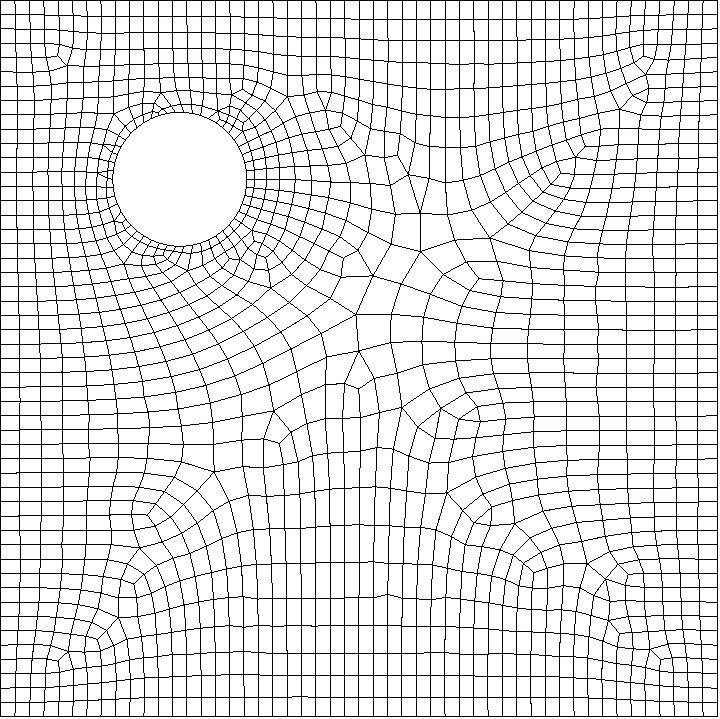
\includegraphics[height=5.0cm]{Chapter_1/figure/conforming_t1.jpg}
	}
	\quad
	\subfigure[Conforming mesh, $t = t_2$]
	{
	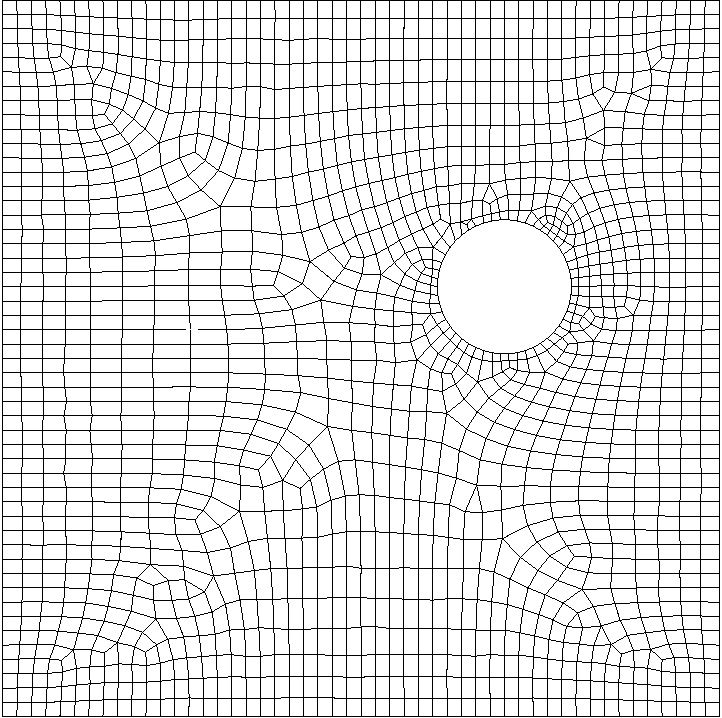
\includegraphics[height=5.0cm]{Chapter_1/figure/conforming_t2.jpg}
	}
	\\
	\subfigure[Nonconforming mesh, $t = t_1$]
	{
	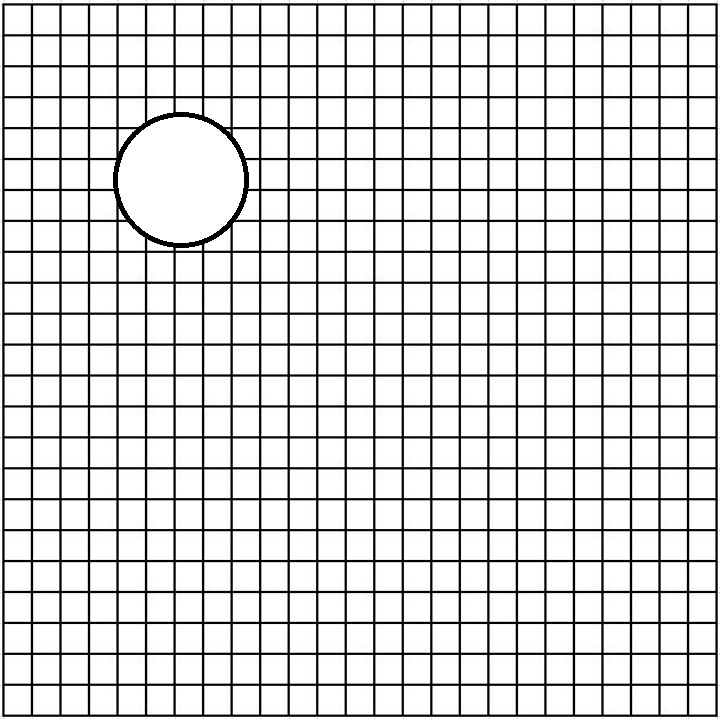
\includegraphics[height=5.0cm]{Chapter_1/figure/nonconforming_t1.jpg}
	}
	\quad
	\subfigure[Nonconforming mesh, $t = t_2$]
	{
	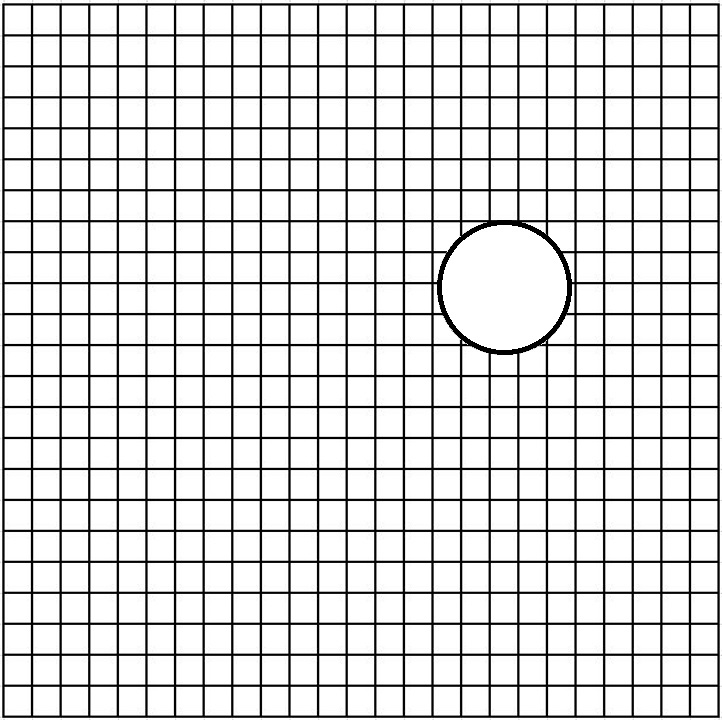
\includegraphics[height=5.0cm]{Chapter_1/figure/nonconforming_t2.jpg}
	}
	\caption{Example of conforming and nonconforming meshes.}
	\label{fig:C1_conformalVSnonconformal}
\end{figure}
%

Non-body conformal Cartesian grid can also be utilized for this simulation as shown in Figure \ref{fig:C1_conformalVSnonconformal}. In this approach the IB would still be represented through some means such as a surface grid, but the Cartesian volume grid would be generated with no regard to this surface grid. Thus, the solid boundary would cut through this Cartesian volume grid. Because the grid does not conform to the solid boundary, incorporating the boundary conditions would require modifying the equations in the vicinity of the boundary. Assuming that such a procedure is available, the governing equations would then be discretized using a finite-difference, finite-volume, or a finite-element technique without resorting to coordinate transformation or complex discretization operators.

Depending on how the effect of solid boundaries are imposed, IB methods can be divided into three categories: i) Continuous forcing, ii) discrete forcing, and iii) cut-cell method.

The continuous forcing method was originally used by Peskin \cite{peskin1977numerical} and later further developed by others researchers \cite{saiki1996numerical, zhu2003interaction, beyer1992analysis}. In this approach, the boundary configuration is described by a curve $x(s,t)$ (Lagrangian nodes) where the location of each point on this boundary is governed by its equations of motion. The forces that the curve $x(s,t)$ exerts on the fluid is calculated by the constitutive law of the curve $x(s,t)$ that relates the displacements to stress values. These stress values are transferred to the Navier-Stokes (NS) (Eulerian nodes) for the fluid by means of a Dirac delta function. Practical implimentation of this method rests in representing the Dirac delta function as a discrete function that has the same properties. This method is applied to a variety of problems, including Cardiac blood flow \cite{peskin1989three}, animal locomotion \cite{fauci1988computational}, multiphase flows \cite{kempe2015imposing}, and particle sedimentation \cite{uhlmann2005immersed}.

Peskin's method is well suited for the elastic boundaries. For stiff boundaries, the constitutive laws of the solid boundaries will result in instabilities in the solution of governing equations \cite{mittal2005immersed}. The virtual boundary method of Goldstein \cite{goldstein1993modeling} enables us to handle these rigid boundaries. The main idea of this approach is the same as Peskin's method where the solid boundary is treated as a virtually existing surface embedded in the fluid. The force on this surface is calculated by the requirement that the fluid velocity should satisfy the no-slip condition. Since this body force is not known a priori, it is calculated in a feedback way.

The penalization method is also categorized under the continuous forcing approaches to the IB problem. This technique is based on the Brinkman equation that describes the fluid flow through a porous medium. The Brinkman equation is analogous to Fourier's laws in heat conduction and Ohm's law in the field of electrical engineering \cite{durlofsky1987analysis}. This approach was first proposed by Arquis and Caltagirone \cite{arquis1984conditions} where they imposed the boundary conditions by adding the penalization terms to the momentum equations. The main idea of this approach is to model the solid obstacles as a porous medium with the porosity of $\mathcal{K}$. The porosity is a measure of the void spaces in a material. Therefore, by selecting low values for porosity, the porous domain acts as a solid wall. It has been demonstrated that the solution of the penalized incompressible NS equations converges to the exact solution as the porosity approaches zero \cite{angot1999analysis} however in the practical implementation, extreme low values for porosity will result in systems with a very large stiffness and numerically unstable. To apply the porosity within the solid domain, a Heaviside function is used by different researchers \cite{gazzola2011simulations, kevlahan2001computation}.

The continuous forcing approach is very attractive for flows for both rigid and elastic boundaries due to its ease of implementation. This technique can be added to an already available commercial package such as ANSYS Fluent for CFX with limited effort. One of the shortcomings of this approach is the smoothing of the forcing function near the boundary. This can result in inability for sharp representation of the immersed boundary in cases such as compressible flows. However, accuracy for representing the boundaries can be improved by refining the mesh and using higher order force mapping schemes.

Mohd-Yusof formulated the discrete formulation of IB method \cite{mohd1997combined} for addressing the time penalties associated with the simulation involving moving boundaries. The main idea of this technique is same as the virtual boundary method where a force term is added to the momentum equations to represent the solid boundary. However, in the current approach the momentum equation manipulation is done in the discrete manner. In the work of Mohd-Yusof \cite{mohd1997combined} and Verzicco et al. \cite{verzicco1998complex} this is done by modifying the discretization stencil in the vicinity of the boundary curve so that the velocity values on this boundary satisfy a pre-defined condition. The major advantage of this approach is the absence of user specified parameters however, its implementation depends strongly on the discretization approach used for the analysis. Therefore, it cannot be easily implemented in commercial codes. This implementation of discrete forcing method has been applied to many different problems such as turbulent flow inside an internal combustion engine \cite{verzicco1998complex}, flow past 3D bluff bodies \cite{verzicco2002large}, and flow in a cylindrical stirred tank \cite{iaccarino2003immersed}.

In the cut-cell methods, the grid cells are cut by the solid boundary and reshaped so that they form a boundary-conforming, unstructured grid. This is shown in Figure \ref{fig:C1_cutCellMesh}.

\begin{figure}[H]
	\centering
	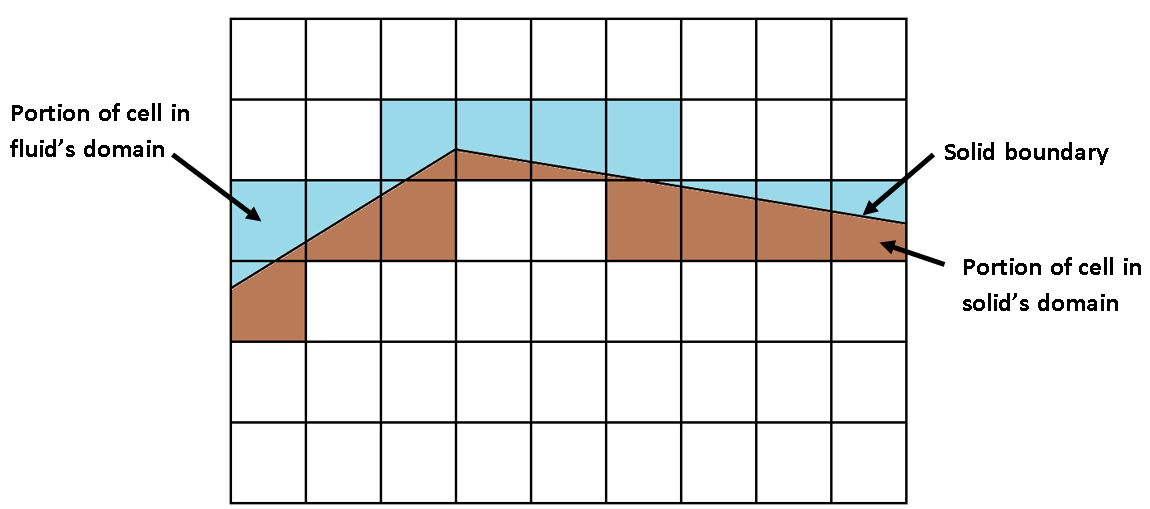
\includegraphics[height=7.0cm]{Chapter_1/figure/cut_cell_mesh}
	\caption{Modified mesh near the solid boundary for cut-cell method.}
	\label{fig:C1_cutCellMesh}
\end{figure}

The cut-cell method was first introduced by Clarke \cite{clarke1986euler} for inviscid flows. This method has been applied to both collocated and staggered grids \cite{kirkpatrick2003representation} however, most of the applications were focused on 2D flows \cite{hu2006conservative, udaykumar1999computation}. This is because of the many possibilities for the geometrical shape of the cut-cell, that makes the flux calculation and therefore numerical implementation extremely difficult.

% ---------------------------------------------------------------------------------------------
\subsection{Sensitivity analysis for IB method}
The body of the research done in the immersed boundary community has been concentrated on the improvement of the method accuracy and resolving the stability issues. However, there has not been much effort in the sensitivity calculation using an IB formulation. There has been some research on the sensitivity analysis using the penalization framework. Borrvall and Petersson applied the penalization method for topology optimization of fluids in Stokes flow \cite{borrvall2003topology}. They used the discrete sensitivity analysis to calculate the sensitivity of fluid pressure to the shape of the boundaries. They used this technique to optimize the shape of a diffuser and also a pipe bend. They verified their methodology for outflow problems as well, where they optimized the shape of solid domain to maintain the least possible pressure drop by constraining the penalized region volume.  Challis and Guest investigated the level set formulation for the topology optimization of fluids in Stokes flow \cite{challis2009level}. They used the penalization technique to formulate the no-slip condition on the solid boundaries. They implemented the topological sensitivities in their solver where they used power dissipation minimization to optimize the shape of a diffuser and a connecting 3D pipe. The penalization method is probably the easiest of the IB methods to implement. This is because it does not have a free parameter such as in virtual boundary method and does not depend on the discretization such as discrete forcing methods. Moreover, no interpolation is needed for applying penalization method to a computational domain. In the penalization method, the fluid and solid domains are differentiated based on a scalar function (porosity) which is very similar to the density based approaches in the topology optimization community \cite{deaton2014survey}. This is probably the biggest reason for researchers to use penalization technique for shape optimization using IB method since the available techniques from topology optimization community can be used \cite{leveque1997immersed, pingen2007topology}. Similar to topology optimization, the shortcoming of penalization technique is in its accuracy for representing the boundaries. Since the nodes are assigned with the porosity values, it is extremly difficult if not impossible to control the exact location of immersed boundary if it does not coincide with the computational nodes. Moreover, the current demonstration problems for the penalization technique are only applicable to low Reynolds numbers flow.

% ---------------------------------------------------------------------------------------------
\section{Research Contribution}
Design optimization for coupled fluid-solid interaction problems is a challenging effort. The current state-of-art technique handles the MDO problem by using unstructured gird and using DSA for sensitivity calculation. However, these techniques cannot be used along with arbitrary software package without a deep underestaning of how the governing equations are formulated and discretized within the solver. Moreover, due to the use of body-conformal grids for fluid domain discretization, additional cost and effort are introduced in both the analysis and sensitivity calculation. Approximating the mesh sensitivities and mesh deformation are two examples for this extra calculation. This research presents a specific formulation for immersed boundary method along the continuum sensitivity analysis for satisfying both of the issues regarding mesh deformation and sensitivity implementation. The specific contributions of this research are as follows

\begin{itemize}
	\item Two different classes of continuous immersed boundary methods are explained and used within CSA framework to calculate the sensitivity of different flow parameters with respect to shape design variables. The immersed boundary method are based on relaxed Dirac delta functions to transfer the data between the fluid and structure domains however, this formulation cannot be used within the CSA framwork. Smooth representation for Dirac delta function is developed for this need.
	\item This research is the first application of CSA for sensitivity analysis of full Navier-Stokes equations. The previous works mainly focoused on Euler and Potential flows where the viscous shear effects are ignored. Using full Navier-Stokes equation, it is possible to reach higher fidelities in design optimization for FSI problems.
	\item The use of continuum immersed boundary methods for sensitivity analysis of flows with moderate to high Reynolds number is another contribution of this work. Most of the work done in this area regarding the sensitivity analysis is based on flows with lower Reynolds number such as Stokes flows.
\end{itemize}
